\documentclass{article}

\title{\lr{Flight Dynamic II Bonus \#1}}

\author{علی بنی‌اسد 96108378}

\usepackage{lipsum}
\usepackage{fancyhdr}
\pagestyle{fancy}
\renewcommand{\sectionmark}[1]{%
	\markboth{\thesection\quad #1}{}}
\fancyhead{}
\fancyhead[R]{\leftmark}
\fancyhead[L]{علی بنی‌اسد 96108378}

\usepackage{graphicx}

\usepackage{xepersian}
\settextfont{B Nazanin}


\begin{document}
	\maketitle
	\section{مقدمه}
	در این گزارش ابتدا به بررسی تاربخچه اثر پرداخته می‌شود سپس به بررسی کارکرد آن از دیدگان مورخین پرداخته خواهد شد. 
	\begin{figure}[h!]
		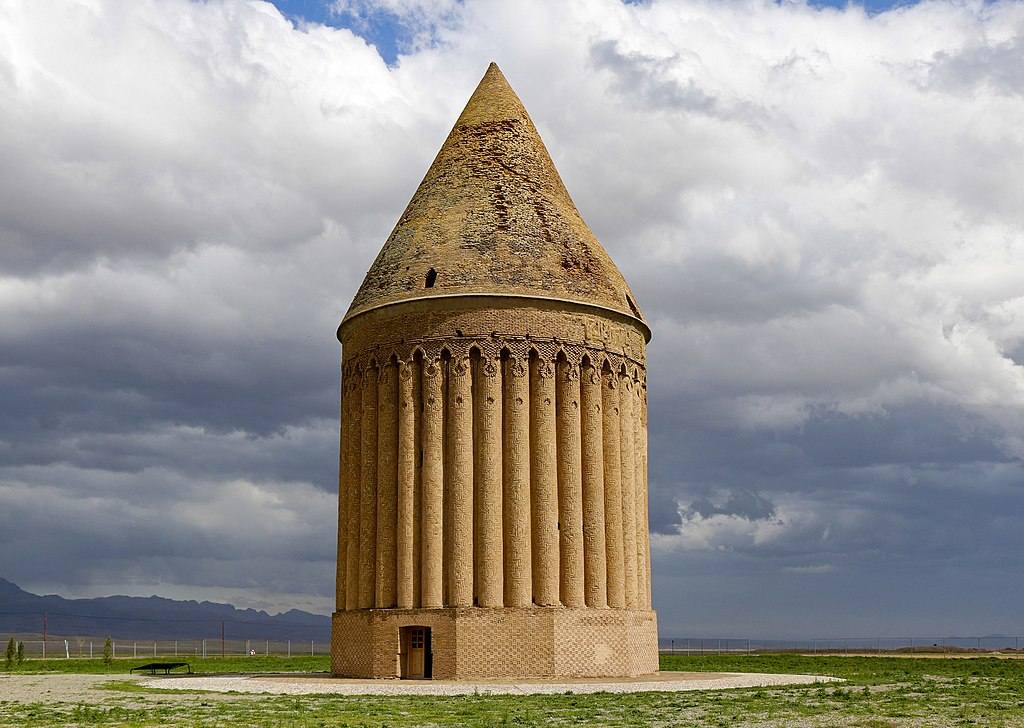
\includegraphics[width=\linewidth]{figures/Radkan_Tower,_Chenaran_2015-01-26.jpg}
		\caption{برج رادکان}
		\label{radkan}
	\end{figure}


در شکل \ref{radkan} نمایی از این برج آورده شده است. برج رادکان یک میل و بنای تاریخی است که در فاصله ۷۴ کیلومتری شمال مشهد و ۲۶ کیلومتری شمال غربی چناران واقع شده‌است. برج رادکان به ارتفاع ۲۵ متر، با بدنه استوانه‌ای و گنبد مخروطی شکل، اثری تاریخی مربوط به قرن هفتم هجری است. نمای خارجی بنا تا ارتفاع سه متری به صورت ۱۲ ضلعی و پس از آن تا زیر گنبد دارای ۳۶ ترک یا نیم استوانه بوده و داخل آن هشت ضلعی است.

\clearpage
برج رادکان چناران بر دشت میان توس و رادکان سایه افکنده و همتای دیگر آن نیز در کردکوی وجود دارد که به رادکان غربی مشهور است. همین موضوع باعث شده برخی نام رادکان را با راه و مسیر هم پیوند بدانند چنان‌که «راد» و «رد» در زبان پهلوی به معنای نظم و ترتیب و «رده» آمده و برج رادکان در مسیر راه و جاده درست همین کار را می‌کند که از نامش پیداست.
\section{معماری}
بلندای این برج ۳۵ متر، قطر داخلی‌اش ۱۴ متر و قطر خارجی آن ۲۰ متر می‌باشد. منظر بیرونی بنا تا ارتفاع ۵.۲ متری به شکل ۱۲ ضلعی و از آن جا تا زیر گنبد به صورت ۳۶ ترک نیم ستونی ساخته شده‌است. برج رادکان دارای گنبد مخروطی شکل است که ساختمان آن احتمالاً در سال ۶۰۷ قمری به پایان رسیده‌است. تاریخ احداث برج رادکان را ماکس افن برشم آلمانی سال ۶۰۰ و اندی و هرتسفلد سال ۶۸۰ ذکر کرده‌اند. هرتسفلد برج را مقبره یکی از حکام مغول می‌داند که برخی وی را امیر ارغون مغول می‌دانند. گدار مستشرق فرانسوی آن را آرامگاه یک زن و مطلع الشمس آن را از آثار دیلمی‌ها می‌داند. علاوه بر راهنمایی مسافران و مقبره به دلیل وجود منفذهایی به تعداد بروج دوازده‌گانه برخی برای این برج کارکرد تقویم و ستاره‌شناسی نیز قائل‌اند. برج رادکان، در روزگار اوج خود، تنها تعیین‌کننده فصل، سال و نوروز در جهان بوده‌است.

در مورد معمار و طراح این اثر اطاعات دقیقی وجود ندارد. در یعضی موارد طراحی برج را به احمد بن عمر نسب داده‌اند در حالی یعضی معتقداند این اثر شاهکار  خواجه نصیرالدین طوسی است.

\section{کارکرد}

\end{document}
